\documentclass[aspectratio=169,12pt]{beamer}

\usepackage{fontspec}
\usepackage{xeCJK}

% math tools
\usepackage{amsmath}
\usepackage{amssymb}
\usepackage{amsfonts}

\usepackage[most]{tcolorbox}
\usepackage{xcolor}

% figures and tables
\usepackage{graphicx}
\usepackage{float}
\usepackage{booktabs}
\usepackage{tikz}
\usetikzlibrary{arrows.meta, positioning, shapes.geometric}

\graphicspath{{../outputs/}}

% Chinese
\xeCJKsetup{AutoFakeBold=true, AutoFakeSlant=true}
\setmainfont{Times New Roman}
\setCJKmainfont{標楷體}

% Beamer theme
\usetheme{Madrid}
\usecolortheme{default}
\setbeamertemplate{navigation symbols}{}
\setbeamertemplate{caption}[numbered]

\title{Phase I/II Statistical Process Monitoring\\SECOM Data}
\author{黃丞暘}
\institute{統計專論 (III) Final Report}
\date{2026/06/16}

\begin{document}

%================================================
\begin{frame}
    \titlepage
\end{frame}

%================================================
\begin{frame}{Project Objective}
    \begin{itemize}
        \item Dataset: UCI SECOM
        \item Objective: Construct SPC workflow % a conflict
        \[
            \text{Phase I} % diagnosis
            \rightarrow
            \text{Control chart design}
            \rightarrow
            \text{Phase II} % monitoring
        \]
        \item Main comparison: Shewhart, EWMA, CUSUM, and CPD charts
        \item Final:
        \begin{enumerate}[1.]
            \item Which chart signals first ?
            \item Whether the pattern suggests mean shift, variance shift, or structural change ?
        \end{enumerate}
    \end{itemize}
\end{frame}

%================================================
\begin{frame}{Selected Variable and Preprocessing}
    \begin{block}{Variable}
        Selected process variable: \textbf{$x_{297}$}
    \end{block}
    \begin{itemize}
        \item Reason: Low missing, High distinct
        \item Samples: 1567
        \item Missing samples removed: 2
        \item Outlier: 1.5 IQR filter after dropping missing values
        \item Outliers removed: 128
        \item Cleaned samples: \textbf{1437}
    \end{itemize}
\end{frame}

%================================================
\begin{frame}{Variable Summary}
    \begin{table}
        \centering
        \begin{tabular}{lrrrrrrr}
            \toprule
            Mean & SD & Min & Q1 & Median & Q3 & Max \\
            \midrule
            1410.91 & 1126.51 & 0 & 556.99 & 1061.44 & 1995.39 & 4945.92 \\
            \bottomrule
        \end{tabular}
    \end{table}
    \begin{figure}
        \centering
        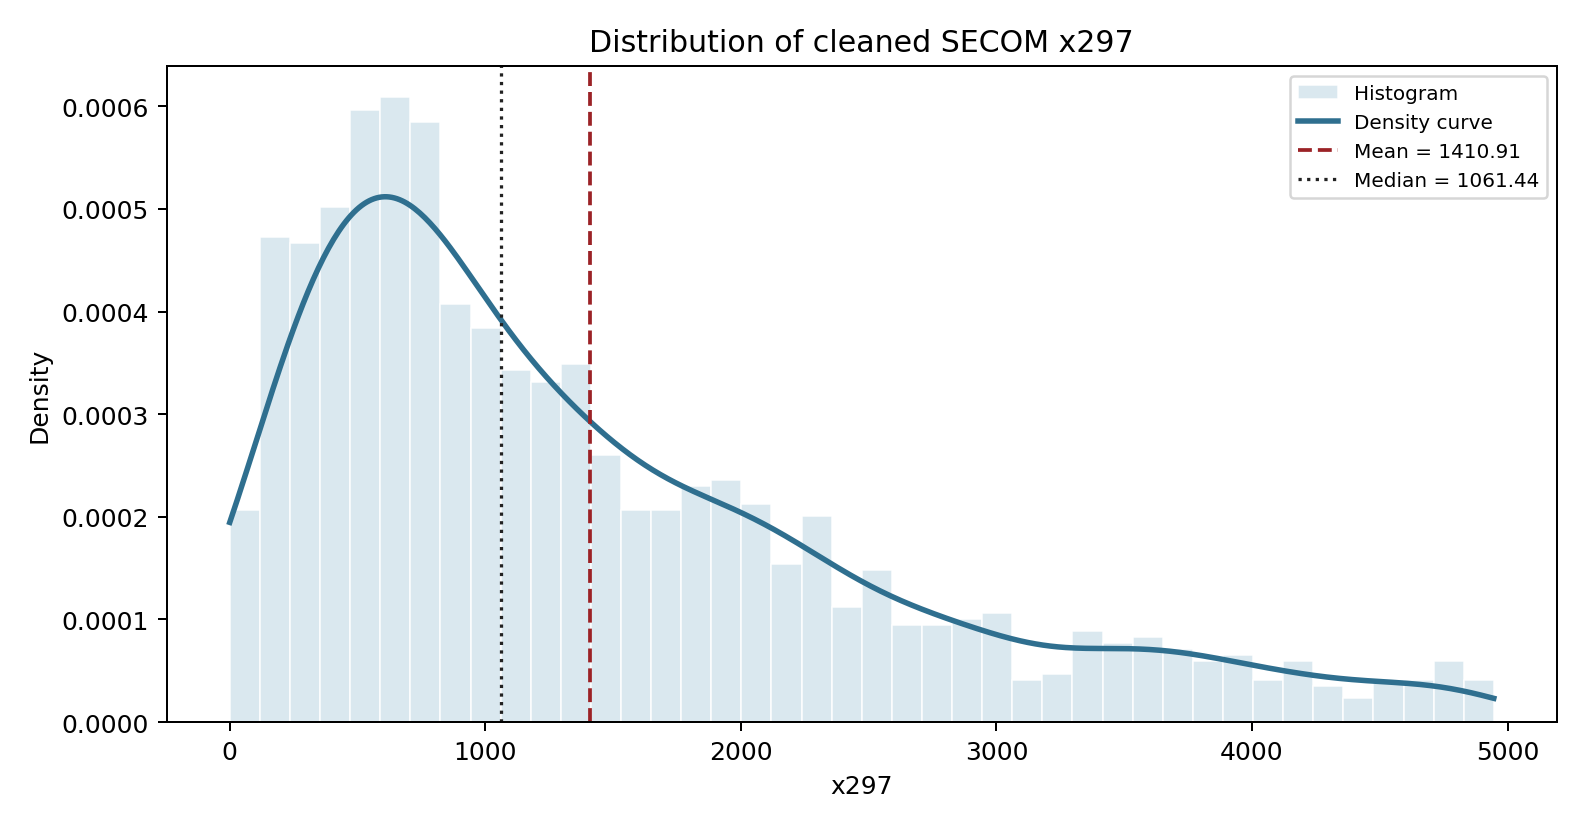
\includegraphics[width=0.7\linewidth]{variable_distribution_x297.png}
    \end{figure}
\end{frame}

%================================================
\begin{frame}{Phase I / Phase II Split}
\[
    m = \lfloor 0.5n \rfloor = \lfloor 0.5(1437) \rfloor = 718
\]
    \begin{table}
        \centering
        \begin{tabular}{lrr}
            \toprule
            Phase & samples & Mean / SD \\
            \midrule
            Phase I & 718 & 1403.64 / 1105.53 \\
            Phase II & 719 & 1418.18 / 1147.80 \\
            \bottomrule
        \end{tabular}
    \end{table}
    \begin{itemize}
        \item Phase I is used as the in-control reference sample
        \item Phase II is monitored sequentially using the chart limits estimated from Phase I
    \end{itemize}
\end{frame}

%================================================
\begin{frame}{Cleaned Series and Phase Split}
\centering
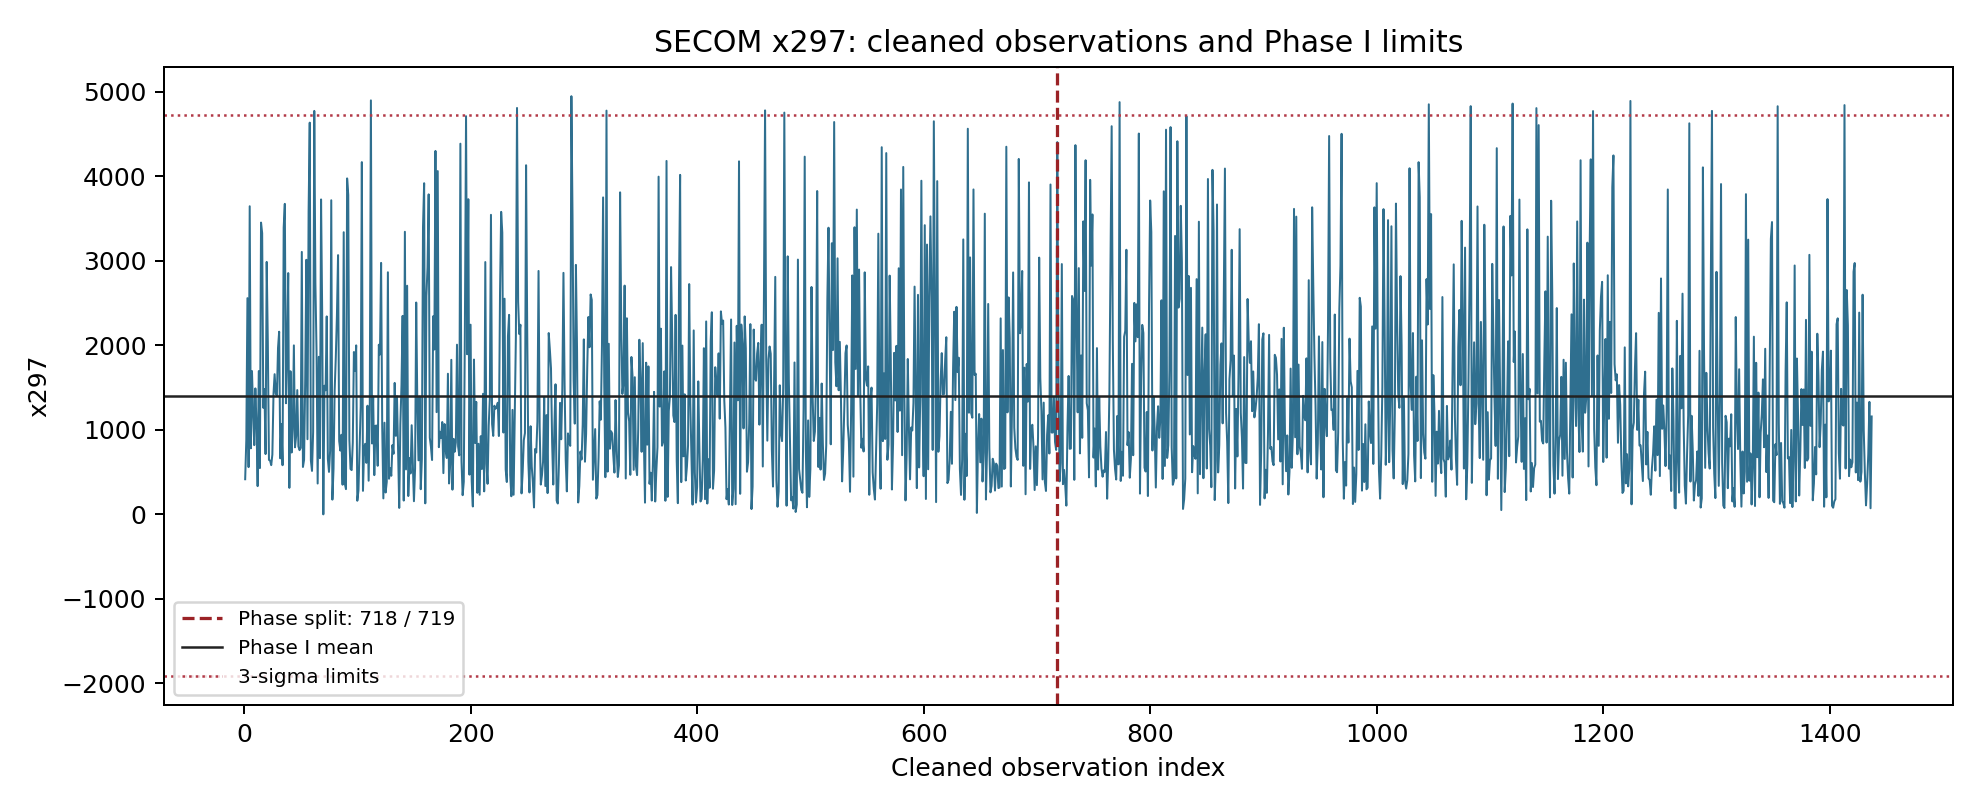
\includegraphics[width=0.94\linewidth]{series_phase_split.png}
\end{frame}

%================================================
\begin{frame}{Phase I RS/P Diagnosis}
\begin{block}{Recursive segmentation + permutation result}
\[
    p_{\text{level}} = 0.8675,\quad
    p_{\text{scale}} = 0.8325
\]
\end{block}

\begin{itemize}
    \item Phase I shows no signifacant evidence of level or scale change
    \item Phase I data can be regarded as stable
\end{itemize}
\end{frame}

%================================================
\begin{frame}{Chart Design}
\begin{table}
\centering
\scriptsize
\begin{tabular}{p{0.28\linewidth}p{0.17\linewidth}p{0.42\linewidth}}
\toprule
Method & Target & Main setting \\
\midrule
Individuals Shewhart & Mean & 3-sigma limits \\
Mean EWMA & Mean & $\lambda=0.1,\ \rho=2.454$ \\
Variance EWMA & Variance & $\lambda=0.1,\ \rho_U=2.595,\ \rho_L=1.580$ \\
Adaptive EWMA & Mean & eta1 case (ii), $h=0.7874$ \\
Mean CUSUM & Mean & $k=0.5,\ h=4.095$ \\
Variance CUSUM & Variance & $k_U=1.848,\ h_U=7.416$; $k_L=0.462,\ h_L=-2.446$ \\
CPD charts & Mean / variance / joint & $\alpha=0.005$ \\
\bottomrule
\end{tabular}
\end{table}

\begin{itemize}
    \item EWMA and CUSUM settings follow the in-class R code.
    \item CPD limits follow Chapter 6 approximations for mean, variance, and joint charts.
\end{itemize}
\end{frame}

%================================================
\begin{frame}{Mean-Shift Monitoring Results {\small (Main Mean Charts)}}

\scriptsize
\renewcommand{\arraystretch}{0.8}

\begin{tabular}{p{0.62\linewidth} p{0.32\linewidth}}

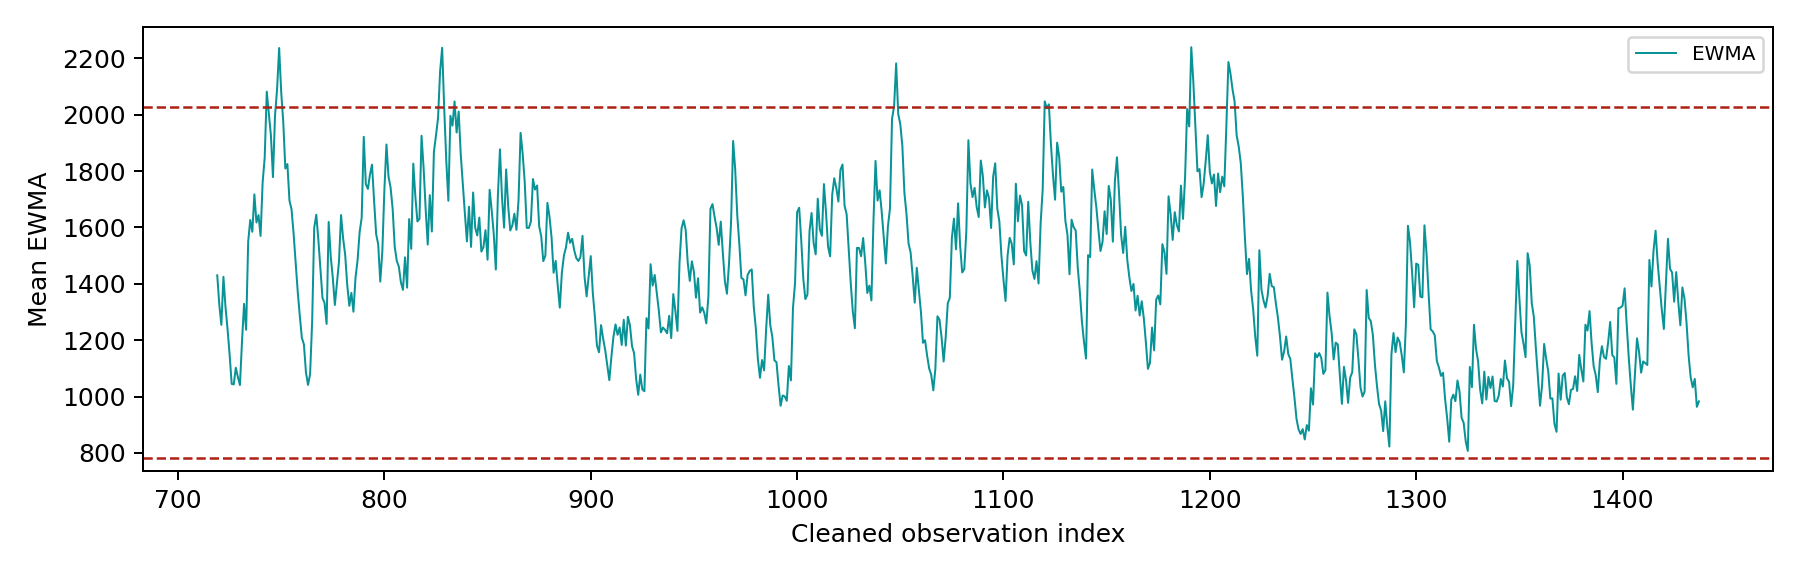
\includegraphics[width=0.5\linewidth]{mean_ewma.png}
&
\textbf{Mean EWMA}\\
First signal: 743\\
Signal count: 17
\\[-0.2em]

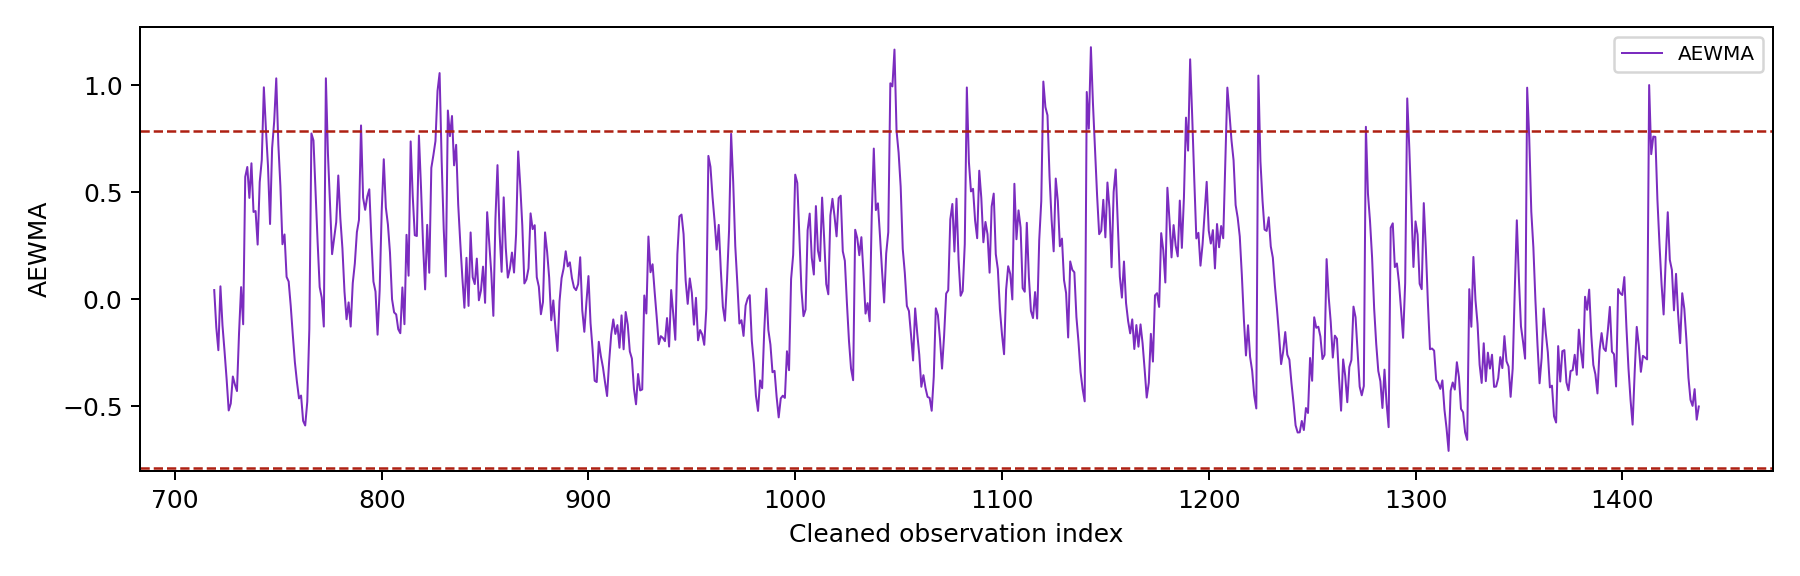
\includegraphics[width=0.5\linewidth]{adaptive_ewma.png}
&
\textbf{Adaptive EWMA}\\
First signal: 743\\
Signal count: 32
\\[-0.2em]

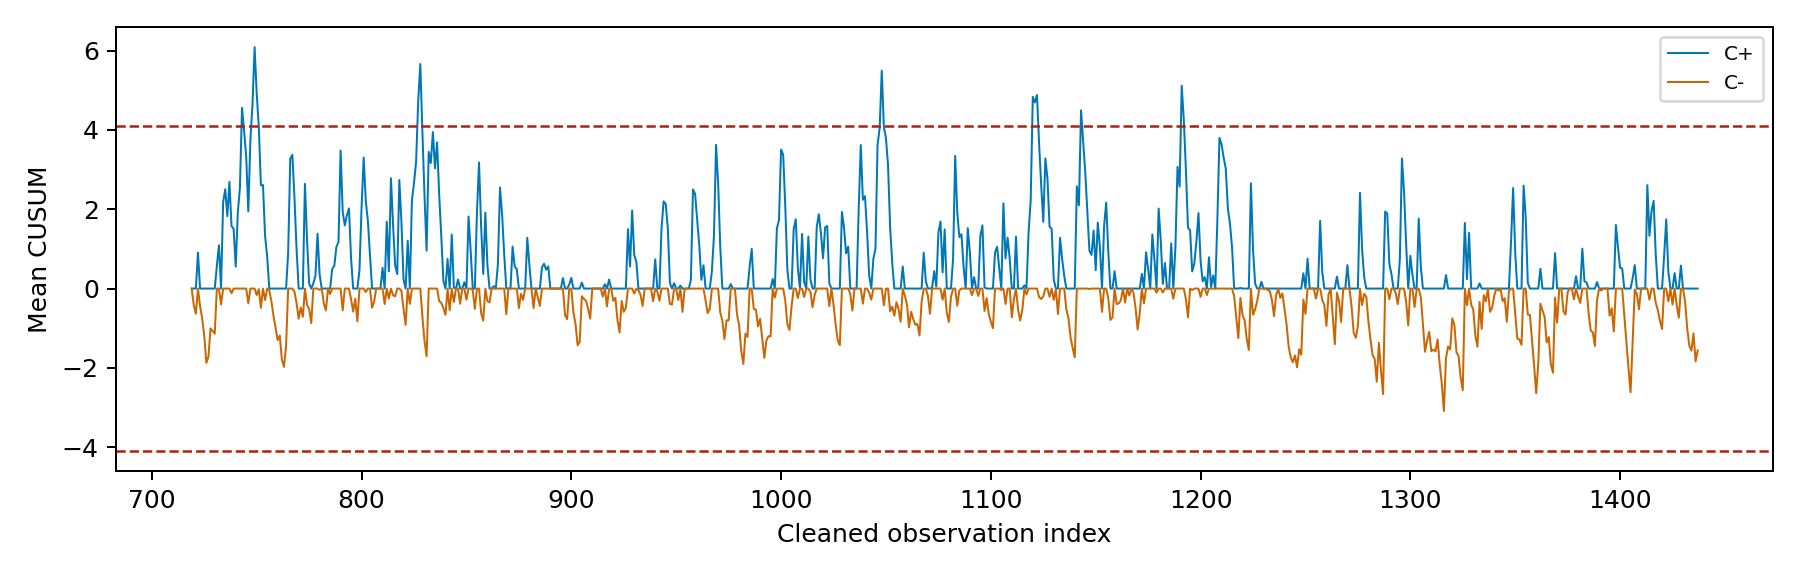
\includegraphics[width=0.5\linewidth]{mean_cusum.png}
&
\textbf{Mean CUSUM}\\
First signal: 743\\
Signal count: 13

\end{tabular}

\end{frame}

%================================================

\begin{frame}{Mean-Shift Monitoring Results {\small (Supplementary Charts)}}

\scriptsize
\renewcommand{\arraystretch}{0.8}

\begin{tabular}{p{0.8\linewidth} p{0.3\linewidth}}
\textbf{Individuals Shewhart}
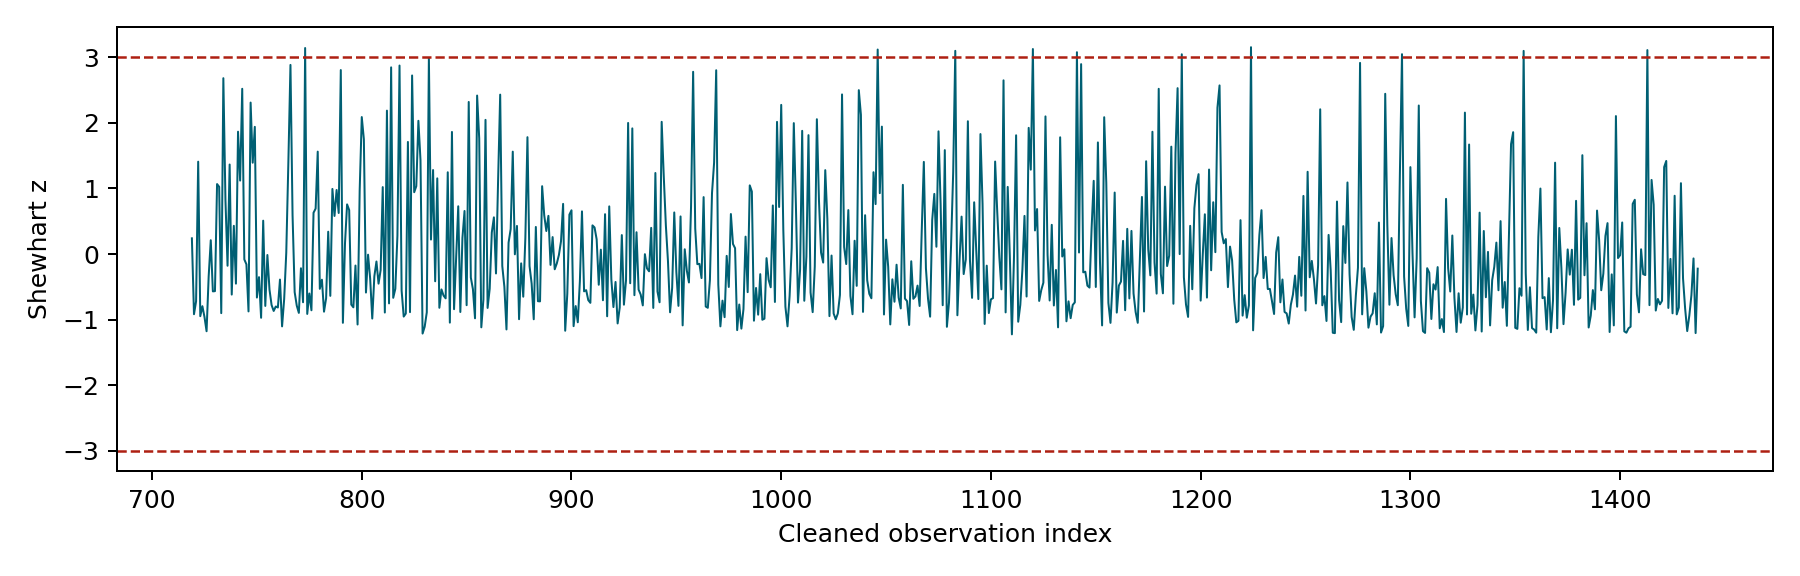
\includegraphics[width=0.8\linewidth]{mean_shewhart.png}
&
\\
First signal: 773\\
Signal count: 10

\textbf{CPD mean chart}
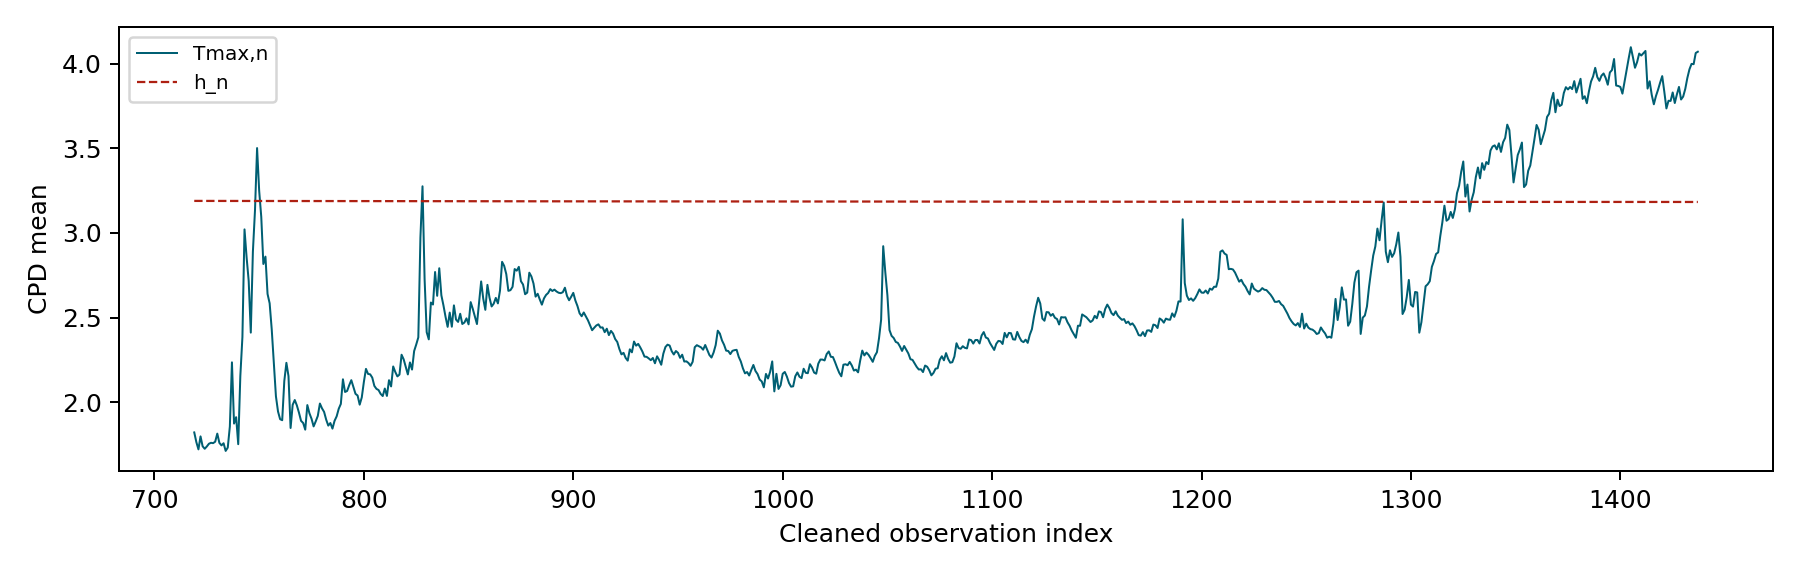
\includegraphics[width=0.8\linewidth]{cpd_mean.png}
&
\\
First signal: 749\\
Signal count: 118

\end{tabular}

\vspace{0.4em}

{\scriptsize
EWMA、AEWMA 與 CUSUM 皆於 743 發出訊號；Shewhart 較晚，CPD mean chart 則顯示較高的訊號頻率。
}

\end{frame}
%================================================
\begin{frame}{Variance-Shift Monitoring Results {\small (Target: Variance)}}

\scriptsize
\renewcommand{\arraystretch}{0.8}

\begin{tabular}{p{0.62\linewidth} p{0.32\linewidth}}

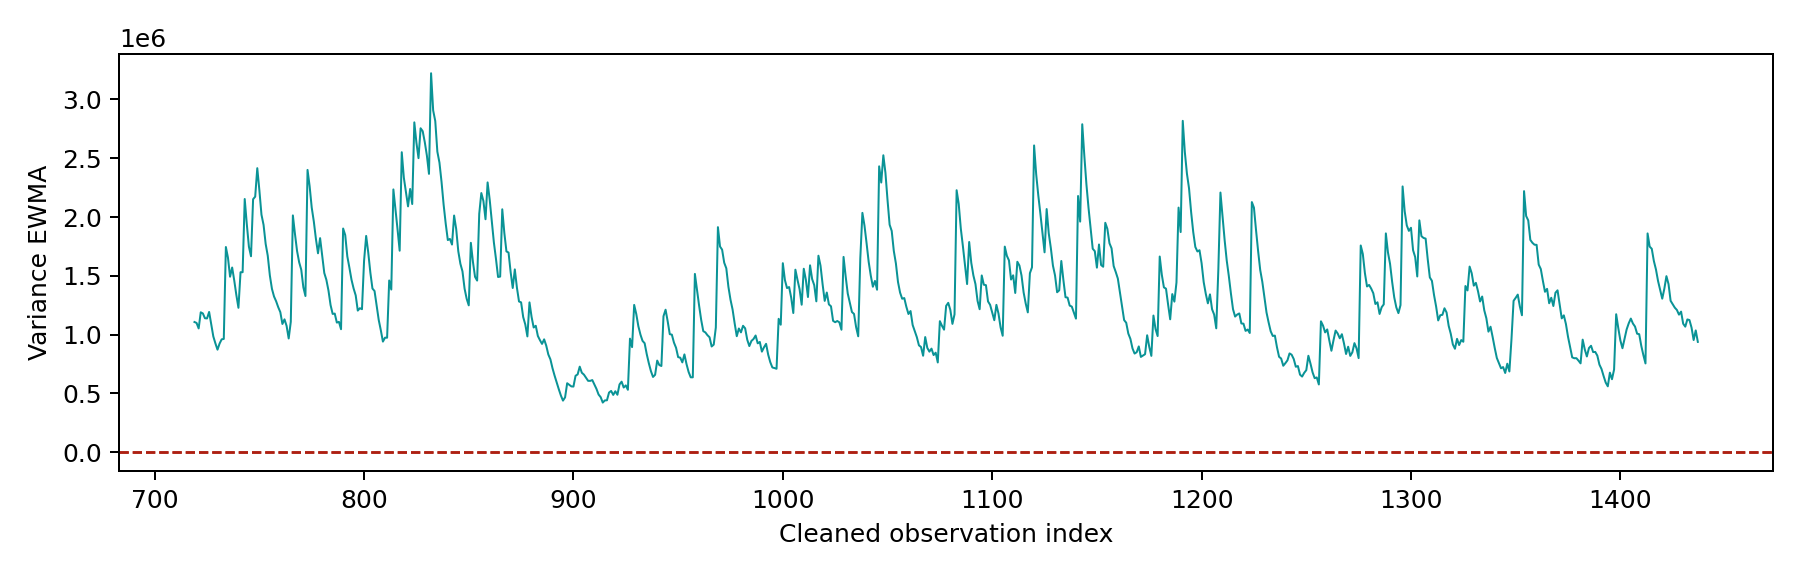
\includegraphics[width=\linewidth]{variance_ewma.png}
&
\textbf{Variance EWMA}\\
First signal: 719\\
Signal count: 719
\\[-0.2em]

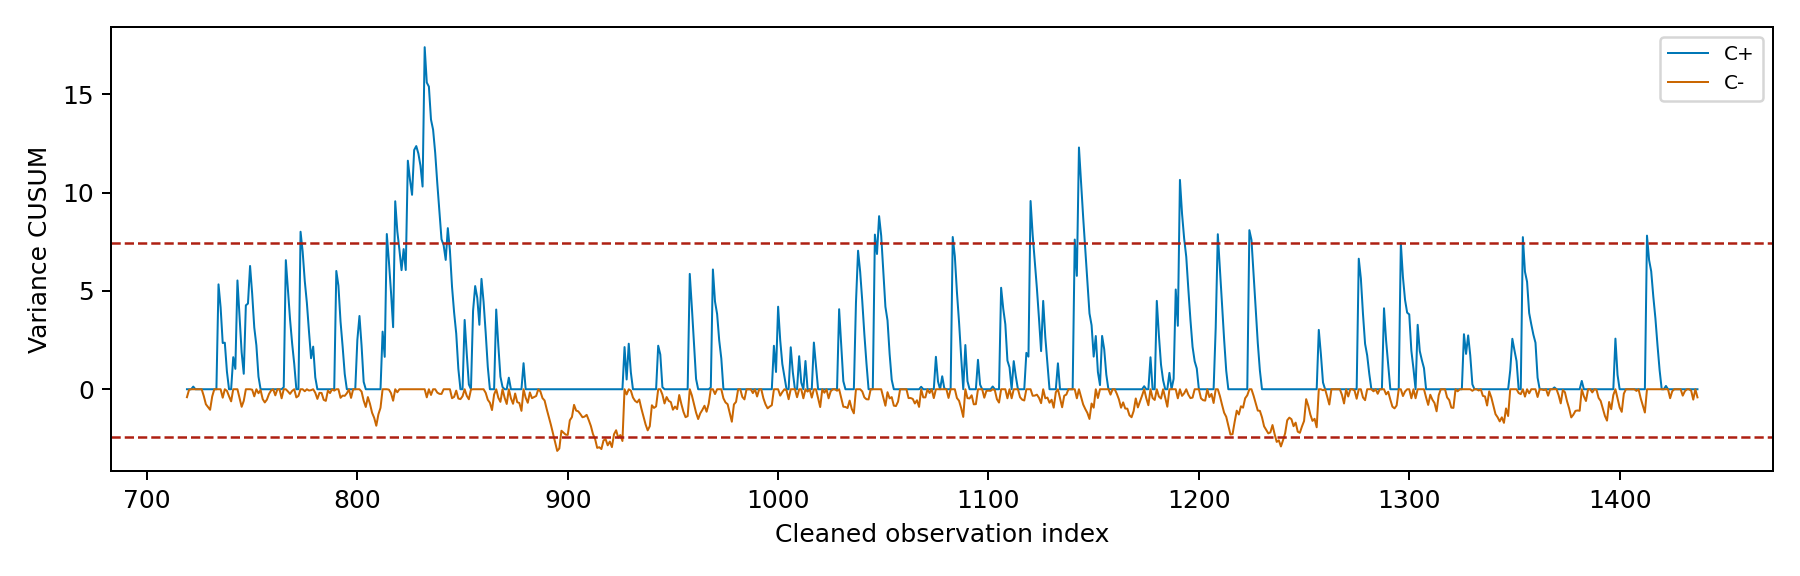
\includegraphics[width=\linewidth]{variance_cusum.png}
&
\textbf{Variance CUSUM}\\
First signal: 773\\
Signal count: 59

\end{tabular}

\vspace{0.4em}

{\scriptsize
Variance EWMA 於 Phase II 第一筆觀測即發出訊號，表示變異數偏移是最早出現的異常型態。
}

\end{frame}
%================================================
\begin{frame}{CPD and Joint Monitoring Results}

\scriptsize
\renewcommand{\arraystretch}{0.8}

\begin{tabular}{p{0.62\linewidth} p{0.32\linewidth}}

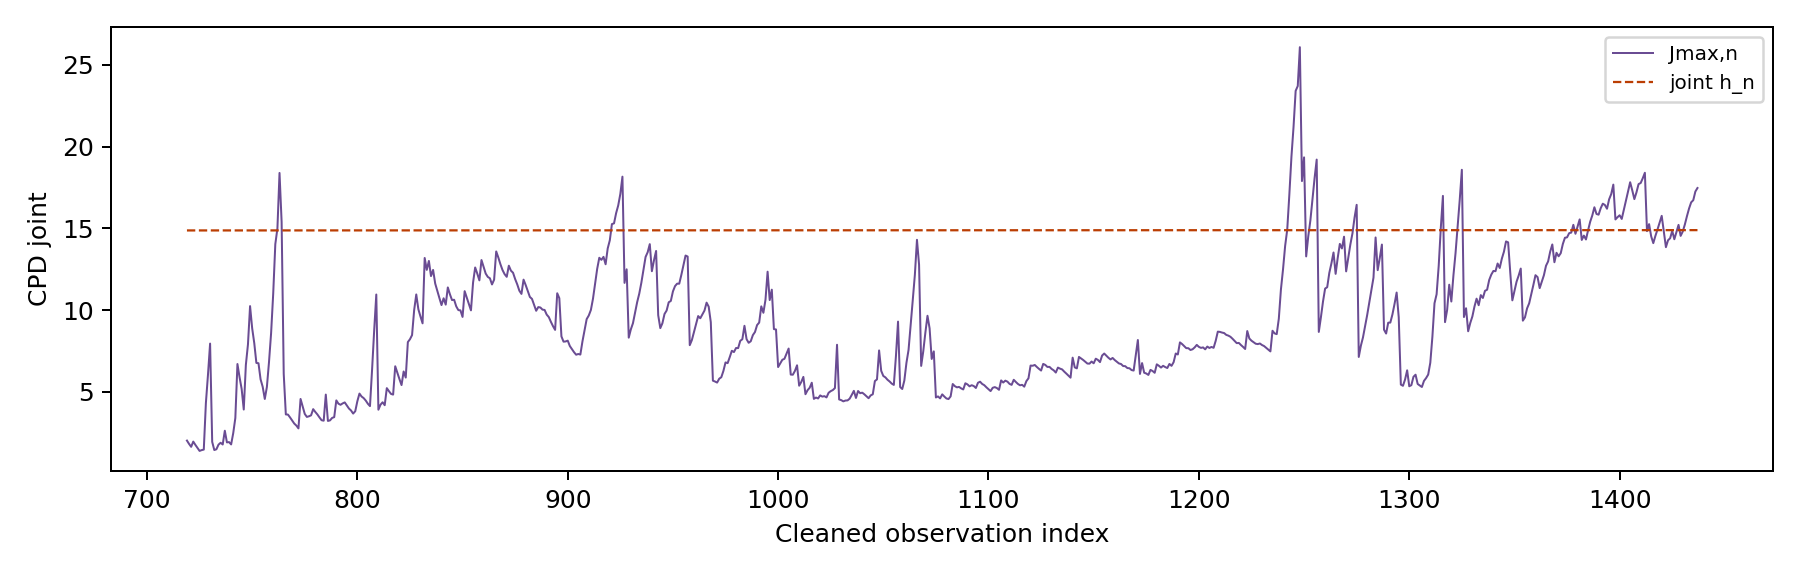
\includegraphics[width=\linewidth]{cpd_joint.png}
&
\textbf{CPD joint chart}\\
First signal: 762\\
Signal count: 71
\\[-0.2em]

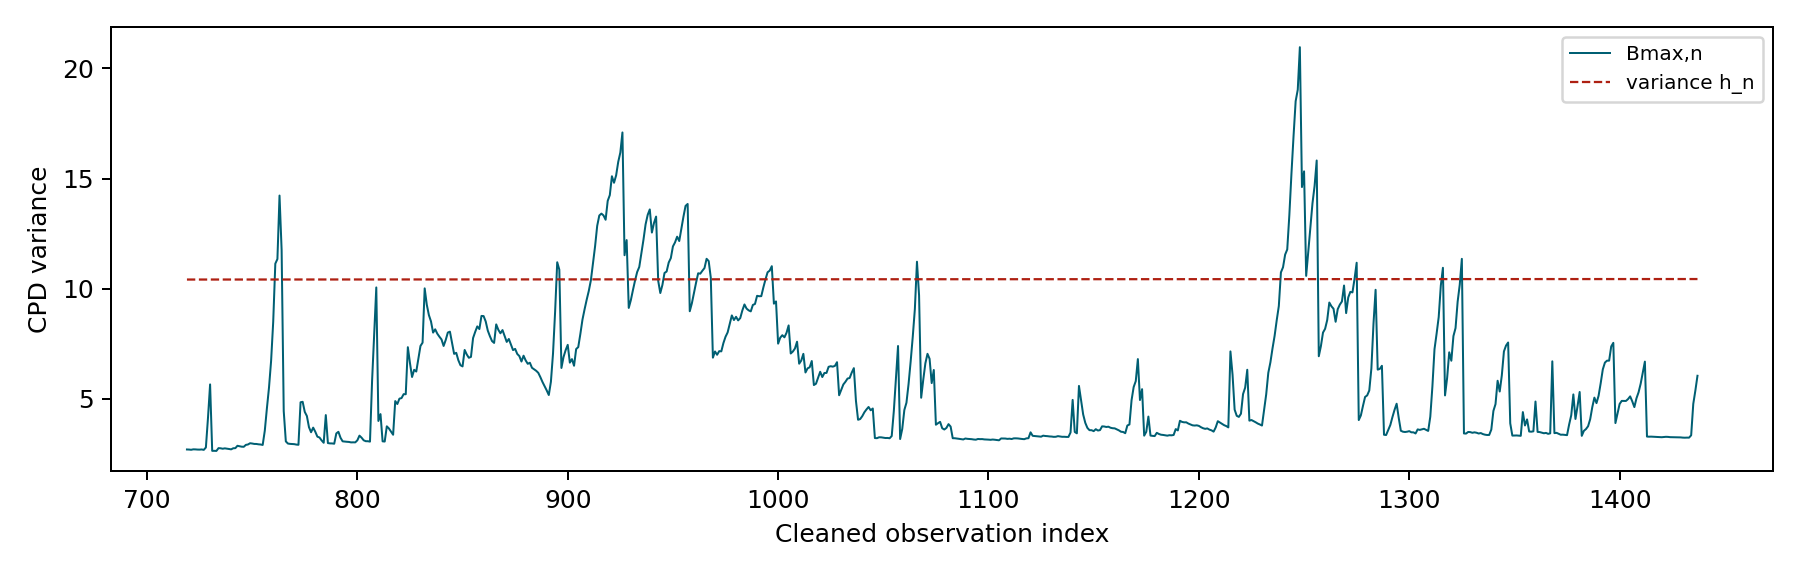
\includegraphics[width=\linewidth]{cpd_variance.png}
&
\textbf{CPD variance chart}\\
First signal: 761\\
Signal count: 78

\end{tabular}

\vspace{0.4em}

{\scriptsize
CPD variance 與 CPD joint chart 的訊號時間接近，表示製程可能同時存在變異數改變與結構性變化。
}

The earliest signal is produced by the variance EWMA chart at index 719,
suggesting that the process change first appears as a variance shift.
Mean-sensitive charts later signal at index 743, indicating that a mean shift
also emerges after the initial variance instability.
CPD-based charts further suggest persistent structural changes in Phase II.

\end{frame}
%================================================
\begin{frame}{CPD Post-Signal Interpretation}
\begin{itemize}
    \item CPD mean chart first signals at index 749
    \item CPD variance chart first signals at index 761
    \item CPD joint chart first signals at index 762
    \item The strongest CPD variance and joint signals estimate the likely change location around:
    \[
        \widehat{r} \approx 1229.
    \]
    \item The strongest CPD mean signal estimates:
    \[
        \widehat{r} \approx 1212
    \]
\end{itemize}
\end{frame}

%================================================
\begin{frame}{Interpretation}
\begin{itemize}
    \item Phase I RS/P diagnosis does not reject stability, so the reference sample is usable.
    \item Phase II mean changes are detected by EWMA, AEWMA, CUSUM, and CPD mean chart.
    \item Variance-sensitive methods are more aggressive, especially variance EWMA.
    \item CPD variance and joint charts locate later structural changes around indices 1229.
    \item Overall pattern suggests not a single isolated mean shift only, but a combination of mean instability and variance/structural change.
\end{itemize}
\end{frame}

%================================================
\begin{frame}{Conclusion}
\begin{enumerate}
    \item The selected SECOM variable $x_{297}$ is usable after missing-value removal and IQR outlier filtering.
    \item Phase I RS/P results support using the first 718 cleaned samples as the IC reference.
    \item The earliest signal is variance EWMA at the first Phase II observation.
    \item For mean-shift detection, mean EWMA, AEWMA, and mean CUSUM signal earliest at index 743.
    \item CPD charts provide additional localization and suggest later structural changes around indices 1212--1229.
\end{enumerate}
\end{frame}

\end{document}
